%% The first command in your LaTeX source must be the \documentclass command.
\documentclass[sigconf]{acmart}





\usepackage{listings}


\lstset{
language=Python,                     % the language of the code
basicstyle=\scriptsize,         % the size of the fonts that are used for the code
backgroundcolor=\color{white},  % choose the background color. You must add \usepackage{color}
showspaces=false,               % show spaces adding particular underscores
showstringspaces=false,         % underline spaces within strings
showtabs=false,                 % show tabs within strings adding particular underscores
frame=single,                   % adds a frame around the code
tabsize=2,                   % sets default tabsize to 2 spaces
captionpos=b,                  % sets the caption-position to bottom
breaklines=true,                % sets automatic line breaking
% breakatwhitespace=false,      % sets if automatic breaks should only happen at whitespace
title=\lstname,                 % show the filename of files included with \lstinputlisting;
                                % also try caption instead of title
escapeinside={\%*}{*)},         % if you want to add a comment within your code
morekeywords={*,...}            % if you want to add more keywords to the set
}

% frame=l,  numbers=left,  numbersep=1em,  xleftmargin=2em



%%
%% \BibTeX command to typeset BibTeX logo in the docs
\AtBeginDocument{%
  \providecommand\BibTeX{{%
    \normalfont B\kern-0.5em{\scshape i\kern-0.25em b}\kern-0.8em\TeX}}}

%% Rights management information.  This information is sent to you
%% when you complete the rights form.  These commands have SAMPLE
%% values in them; it is your responsibility as an author to replace
%% the commands and values with those provided to you when you
%% complete the rights form.
\setcopyright{acmcopyright}
\copyrightyear{2022}
\acmYear{2022}
\acmDOI{XXXXXXX.XXXXXXX}

%% These commands are for a PROCEEDINGS abstract or paper.
% \acmConference[Conference acronym 'XX]{Make sure to enter the correct
%   conference title from your rights confirmation emai}{June 03--05,
%   2018}{Woodstock, NY}
% \acmPrice{15.00}
% \acmISBN{978-1-4503-XXXX-X/18/06}


%%
%% Submission ID.
%% Use this when submitting an article to a sponsored event. You'll
%% receive a unique submission ID from the organizers
%% of the event, and this ID should be used as the parameter to this command.
%%\acmSubmissionID{123-A56-BU3}

%%
%% The majority of ACM publications use numbered citations and
%% references.  The command \citestyle{authoryear} switches to the
%% "author year" style.
%%
%% If you are preparing content for an event
%% sponsored by ACM SIGGRAPH, you must use the "author year" style of
%% citations and references.
%% Uncommenting
%% the next command will enable that style.
%%\citestyle{acmauthoryear}

%%
%% end of the preamble, start of the body of the document source.
\begin{document}

%%
%% The "title" command has an optional parameter,
%% allowing the author to define a "short title" to be used in page headers.
\title{A High-Performance Stream Processing System Implementation for Monitoring Stock Market Data Stream}


\author{Kevin Li, Daniel Fernandez, David Klingler, Yuhan Gao, Jacob Rivera, Kia Teymourian}
\affiliation{
  \institution{The University of Texas at Austin}
  \city{Austin, TX}
  \country{USA}}
\email{{kevinali, daniel.fernandez, davidklingler, yg6952, jacobrivera}@utexas.edu, kiat@cs.utexas.edu}


\begin{abstract}
High-performance monitoring of the stock market data stream is one of the challenging use cases of 
the data stream processing systems. Different continuous queries can be defined by market brokers to provide 
buy and sell advice. 
In this paper, we describe our implementation of a system for the DEBS2022 Grand Challenge to extract 
breakout patterns from real-time stock market data to provide buy and sell notifications. Breakout patterns 
are specified based on long intervals of 50 days and 100 days known as the golden cross to indicate a golden 
opportunity for long-term investments. We report details of our high-performance implementation to extract such 
patterns in real-time be able to generate real-time buy and sell notifications.
\end{abstract}

%%
%% The code below is generated by the tool at http://dl.acm.org/ccs.cfm.
%% Please copy and paste the code instead of the example below.
% %%
% \begin{CCSXML}
% <ccs2012>
%  <concept>
%   <concept_id>10010520.10010553.10010562</concept_id>
%   <concept_desc>Computer systems organization~Embedded systems</concept_desc>
%   <concept_significance>500</concept_significance>
%  </concept>
%  <concept>
%   <concept_id>10010520.10010575.10010755</concept_id>
%   <concept_desc>Computer systems organization~Redundancy</concept_desc>
%   <concept_significance>300</concept_significance>
%  </concept>
%  <concept>
%   <concept_id>10010520.10010553.10010554</concept_id>
%   <concept_desc>Computer systems organization~Robotics</concept_desc>
%   <concept_significance>100</concept_significance>
%  </concept>
%  <concept>
%   <concept_id>10003033.10003083.10003095</concept_id>
%   <concept_desc>Networks~Network reliability</concept_desc>
%   <concept_significance>100</concept_significance>
%  </concept>
% </ccs2012>
% \end{CCSXML}

% \ccsdesc[500]{Computer systems organization~Embedded systems}
% \ccsdesc[300]{Computer systems organization~Redundancy}
% \ccsdesc{Computer systems organization~Robotics}
% \ccsdesc[100]{Networks~Network reliability}

% %%
%% Keywords. The author(s) should pick words that accurately describe
%% the work being presented. Separate the keywords with commas.
% \keywords{datasets, neural networks, gaze detection, text tagging}

%% A "teaser" image appears between the author and affiliation
%% information and the body of the document, and typically spans the
%% page.
% \begin{teaserfigure}
%   \includegraphics[width=\textwidth]{sampleteaser}
%   \caption{Seattle Mariners at Spring Training, 2010.}
%   \Description{Enjoying the baseball game from the third-base
%   seats. Ichiro Suzuki preparing to bat.}
%   \label{fig:teaser}
% \end{teaserfigure}

\maketitle



\section{Introduction}
The algorithmic trading of stock shares can be triggered by high complex event patterns that are specified 
based on patterns in the event stream of the stock market. Such algorithmic trading mostly is specified 
based on the history of the event stream, for example, by utilizing moving averages of stock prices and the trading volumes. 
The real-time extraction of such complex patterns to trigger buy or sell trading actions is the task 
of high-performance event stream processing systems. 

% Describe briefly what the challenge is 
This year's DEBS Grand Challenge \cite{debs2022challenge} describes a system implementation based on two specific queries on the 
stock market event streams. The first query is defined to compute the Exponential Moving Average (EMA) with two 
different smoothing factors of 38 and 100. 
An exponential Moving Average is one of the moving averages and is defined as follows:

\begin{align*}
    EMA_t = \begin{cases} 
        Y_0 &  t = 0 \\ 
        \alpha Y_t + (1-\alpha) EMA_{t-1}& t>0 \\ 
        \end{cases}
\end{align*}

The coefficient $\alpha$ represents the degree of weighting decrease, a constant smoothing factor between 0 and 1.
For this challenge $\alpha = \frac{2}{1+j}$ where $j$ is a smoothing factor with $j \in \{38, 100 \}$.
We use $EMA_{38}$ to refer to the exponential moving average with a smoothing factor of 38 
and $EMA_{100}$ for a smoothing factor of 100. 


\begin{figure}[!ht]
    \begin{center}
        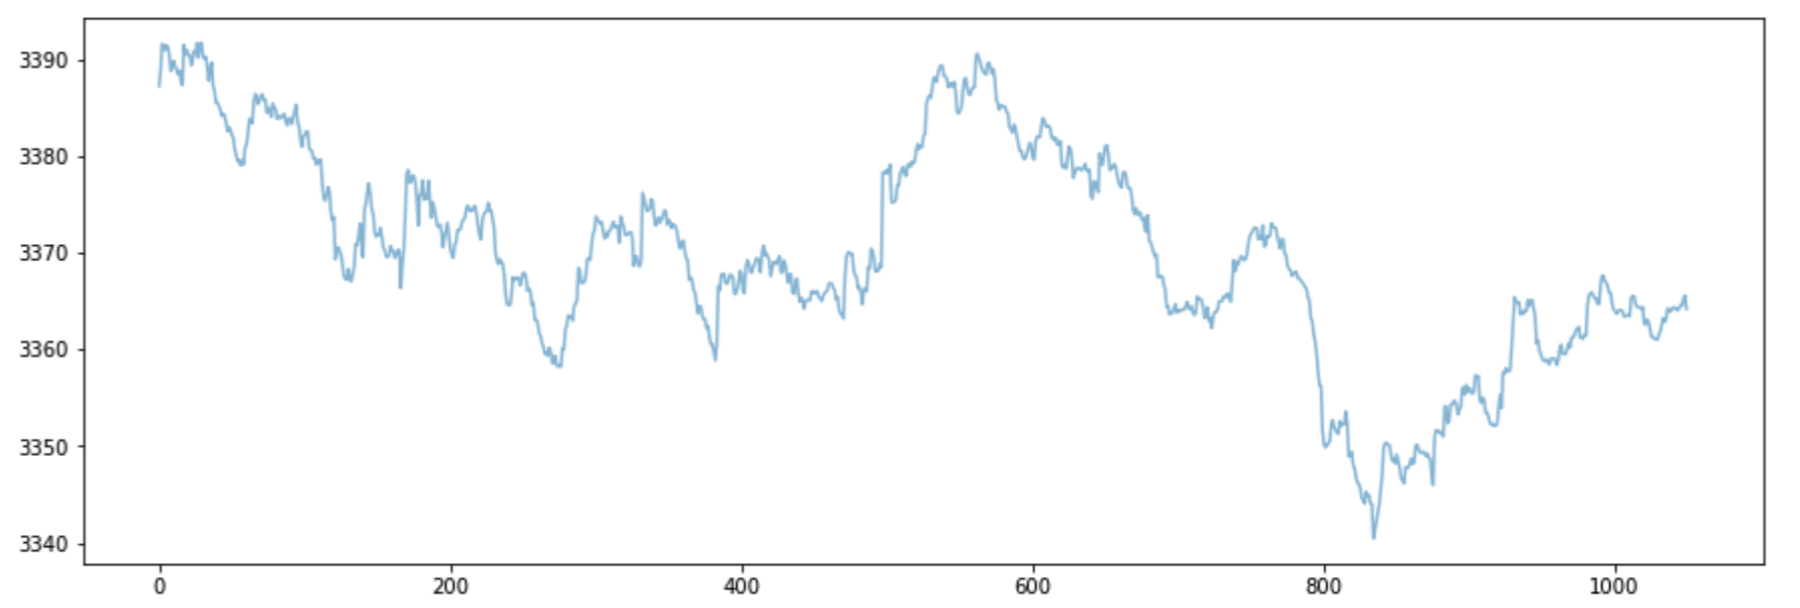
\includegraphics[width=0.42\textwidth]{./images/stock_example.png}
        \caption{An Example of Stock Price Fluctuations Over Time}
        \label{fig:stock}
    \end{center}
\end{figure}



\begin{figure*}[!ht]
    \begin{center}
        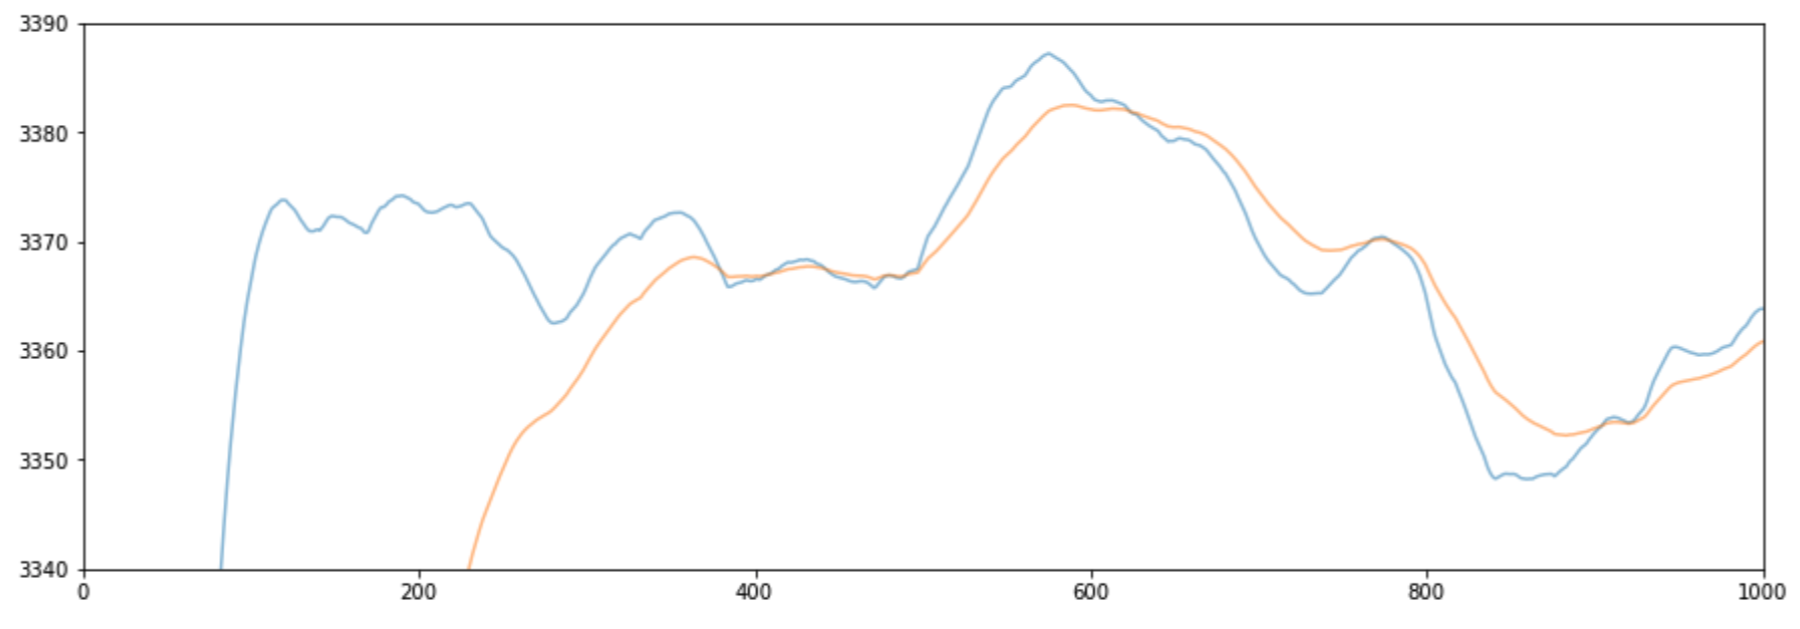
\includegraphics[width=0.70\textwidth]{./images/query2_example.png}
        \caption{Example of Query 2 - Buy and Sell advice based on Breakout Patterns of EMA 38 and 100 }
        \label{fig:EMAs}
    \end{center}
\end{figure*}


% Describe the query 1 and 2 
Figure \ref{fig:stock} illustrates an example of stock market price changes over time. The graph shows 1000 events with 
different prices. Figure \ref{fig:EMA200} depicts the values of the exponential moving average with 
smoothing factors of 38 and 100. We can observe in Figure \ref{fig:EMA200} how the value grows exponentially 
and how the two $EMA_{38}$ and $EMA_{100}$ are different from each other. 

Query 2 of the DEBS2022 challenge \cite{debs2022challenge} is specified based on the results of query 1. Each time 
that $EMA_{38}$ breaks out of the value of $EMA_{100}$ a stock buy advice notification should be generated and if
$EMA_{100}$ goes under the $EMA_{38}$ a stock sell advice. For a further detailed description of the DEBS 2022 
Grand Challenge, we would refer the readers to \cite{debs2022challenge}. 

Figure \ref{fig:EMAs} visualize the same graph as we have in Figure \label{fig:EMAs} by 
zooming into the graph (range 0 to 200 events on x-axis) to see the values and their differentiations. One important observation in 
Figure \ref{fig:EMA200,fig:EMAs} is that $EMA_{38}$ and $EMA_{100}$ have a large difference in the first 
200 events.  The reason for this difference is that the exponential moving average is specified based 
on the history of events to increase the value exponentially and requires a warm-up phase. Based on this observation,
one can improve the performance of the query 2 by skipping the first 200 events for query 2 because 
$EMA_{38}$ and $EMA_{100}$ have still a large difference. 

The main system development challenge task is to design a system that can process the stream of events with high throughput and low latency. 
Many open source and commercial stream processing systems are developed that one can use to develop this challenge. 
Esper event stream processing system \cite{Bernhardt2007} is a system that can detect complex events based on pre-defined temporal logic patterns. 
In this task we do not have a complex pattern to extract and computation are basic computation of EMA 38 and 100, and a subsequent check if the values for 
query 2 to submit a sell or buy advice. Other systems like Apache Storm \cite{8288619}, Apache Spark Streaming \cite{zaharia2010spark} or 
Apache Flink streaming \cite{alexandrov2014stratosphere} are developed to achieve high-scalability in processing the data stream. 
Also, different benchmarks are developed  \cite{8701904} which compare these systems with each other regarding specific data 
stream processing tasks. 

After considering all of the existing systems and their overhead trade-offs, we decided to implement the DEBS grand challenge from scratch and 
without using any of the existing systems because most of them have a different target with a large start-up delay which might impact 
our stream processing performance. The first implementation is a prototype of the system in python because we would like to make sure 
that we understand the logic of these two queries and can run tests to check if the data streams are processed correctly, and the correct 
trading advices are submitted to the DEBS2022 evaluation system. 


% High-Performance computing problems 
% Scalability issues 

\begin{figure}[!ht]
    \begin{center}
        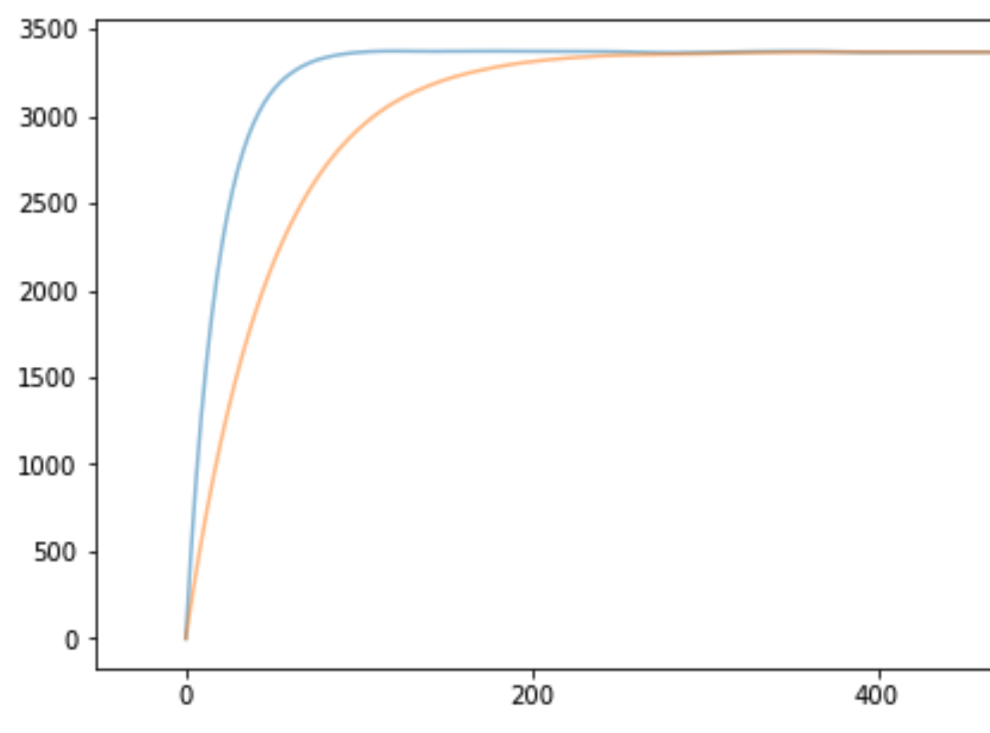
\includegraphics[width=0.4\textwidth]{./images/query2_example_200.png}
        \caption{Exponential Moving Average of 38 and 100 for the first 400 events.}
        \label{fig:EMA200}
    \end{center}
\end{figure}


The next subsequent sections describe details of our implementation. Section \ref{sec:concepts} describes our ideas for 
stream processing using multiple processing threads on a single machine with multiple CPU cores. Further we describe how the same 
architecture can be extended to process the data stream on a cluster of machines.  Section \ref{sec:implementation} provides 
a brief description of important implementation details and Section \ref{sec:experiments} provides a brief overview of different 
experiments.


\begin{figure*}[h]
    \begin{center}
        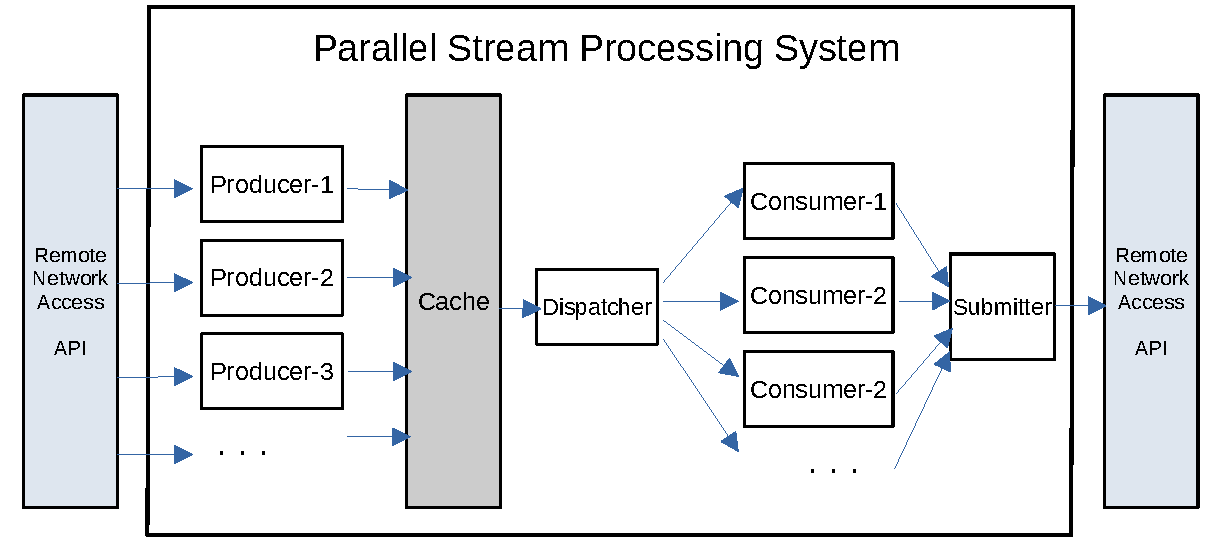
\includegraphics[width=0.6\textwidth]{./images/Parallel-Stream-Processing-System}
        \caption{Event Dispatcher and Submitter Architecture}
        \label{fig:parallel-srream-processing}
    \end{center}
\end{figure*}



\section{Stream Processing Architecture}\label{sec:concepts}
% Describe different ideas for distribution of events on multiple threads/processing and machines.
Our data stream processing architecture is based on the event producers and consumers concept that can be used to distribute the
processing tasks to multiple threads (on a single machine), or separated processes
(distribution on many commodity machines), or a combination of both.
Figure \ref{fig:parallel-srream-processing1} depicts our system architecture. The producers read the data stream batches from the
remote network API (provided by DEBS 2022 Challenge \cite{debs2022challenge}), and store them in a buffer queue in main memory.
The buffer queue has a specific size limitation that can be configured based on the available machine's RAM. The producer will read the data batches
and store them in the queue until the queue size reaches the specific size limit. Once the queue limit is reached, the producer thread or process
is suspended until the queue is available again to receive data. We can use a lock-free queue to cache the incoming data stream before the main processing step.

The processing consumers access batches from the queue and process the events to generate Query 1 (values of $EMA_{38}$ and $EMA_{100}$)
and the subsequent Query 2 results. For the computation of $EMAs$, each consumer is required to know about the
last $EMA$ value of the previous batch for a given stock symbol.
These consumer processes are the major query processing units that we call consumers for the sake of simplicity in this paper.


To make sure that there is no single bottleneck or synchronization lock point in this processing architecture, we made each of the consumers
(processing units) be responsible for the monitoring and the computation of a sub-set of stocks symbol. Each consumer accesses the stream batches
from the main memory cache and processes only the symbols (stock market data events) that this consumer is responsible for.
This can be implemented by using hash functions on stock symbol and mapping it to the unique identification number of the consumer.
In our implementation, the hashing and distribution of the symbols to the consumers is processed in parallel by the producers.

Each consumer has a hash table that it uses to memoize the previous values of the moving averages for different stock symbols. In order to optimize 
for memory and time complexity, the only data stored per symbol include: the latest event (closing price) for the current window, the $EMA_{38}$ and $EMA_{100}$ of 
the previous window, and the last three crossover events.
Each consumer has to access events of each batch and compute those stock symbols that the consumer is responsible for. With this approach, each consumer 
can work independently of any other consumer in a functional form. Access to each data batch from the queue should be implemented in an efficient manner so that each 
consumer does not read the entire batch to filter out the stock symbols it is responsible for.



\begin{figure}
    \begin{center}
        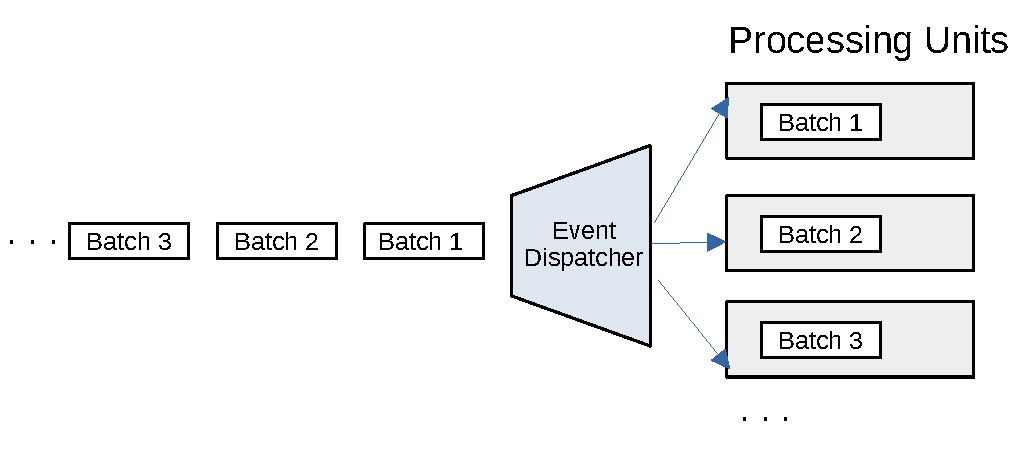
\includegraphics[width=0.43\textwidth]{./images/Stream-Batch-Distributions}
        \caption{An Event Data Dispatcher}
        \label{fig:batch-distributions}
    \end{center}
\end{figure}

Figures \ref{fig:parallel-srream-processing} and \ref{fig:batch-distributions} illustrate the system design if we have included an event dispatcher and 
an event submitter. We do not have a dispatcher and submitter because of efficiency reasons and because of the correctness of query processing. If we dispatch the 
event batches as shown in Figure \ref{fig:parallel-srream-processing}, for example, by round-robin batch distribution, then each consumer has to work on all stock symbols or a subset of them.

If consumers work on all of the events, then each consumer is required to know the previous moving averages from the immediate past batch to compute the new $EMAs$ for
the current data batch; implying a strict dependence on the preceding consumer before the current consumer can proceed. This issue would cause incorrect processing, because a 
consumer should work in a parallel distributed design, without any dependencies on each other's results. In the former case, if the consumers work on a subset of stocks, we would 
need to pass every batch to all of the consumers, and it is better to do this task in an integrated form with reading from the queue.



\begin{figure*}
    \begin{center}
        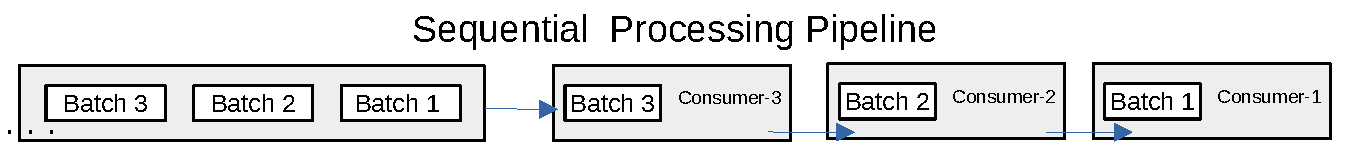
\includegraphics[width=0.7\textwidth]{./images/Stream-Batch-Distributions_op2}
        \caption{A Sequential Processing Pipeline. Each consumer reads a batch and passes to the next consumer.}
        \label{fig:Sequential-batch-distributions}
    \end{center}
\end{figure*}

Figure \ref{fig:Sequential-batch-distributions} illustrates how sequential data stream processing can work to process the batches in multiple
serial event consumers. Each processing unit will pick up and process a subset of stock market events.
In a single machine setup, the overhead of passing the event batches to the next consumer is very small, but in a distributed setting, the
overhead of passing data batches to the next consumer over the network is very high because of data serialization costs. Comparing the
architecture of Figure \ref{fig:Sequential-batch-distributions} and \ref{fig:parallel-srream-processing}, we preferred to implement the system
parallel format shown in Figure \ref{fig:parallel-srream-processing}.


If the stream of data is terminated, the stream processing system will terminate, as producers cannot generate more event batches
 and there are no event batches in the buffer queue.






%%%%%%%%%%%%%%%%%%%%%%%%%%%%%%%%%%%%%%%%%%%%%%%%%%%%%%%%
%%%%%%%%%%%%%%%%%%%%%%%%%%%%%%%%%%%%%%%%%%%%%%%%%%%%%%%%
%%%%%%%%%%    Implementation Details %%%%%%%%%%%%%%%%%%%
%%%%%%%%%%%%%%%%%%%%%%%%%%%%%%%%%%%%%%%%%%%%%%%%%%%%%%%%
%%%%%%%%%%%%%%%%%%%%%%%%%%%%%%%%%%%%%%%%%%%%%%%%%%%%%%%%




\section{Data Stream Windowing}\label{sec:windows}
Based on DEBS Challenge \cite{debs2022challenge} description, our system has to compute on events grouped into windows of 5 minute length, tumbling,
non-overlapping windows. The system clock timer starts when it receives the first event and restarts every 5 minutes. As a preprocessing step, our system reads the events
into main memory and generates data batches, which are then cached. The data batches are thereafter passed to the next processing step for the subsequent computation.
    
    
\section{Implementation Details}\label{sec:implementation}
The described architecture can be implemented using multiple threads on a single machine with multiple CPUs, or it can be distributed over a cluster of machines, each with multiple CPU cores.
Our first rapid alpha implementation of the system was a multi-threaded Python implementation to make sure that we understood the challenge tasks and are able to process the queries in the correct form.
Later, we implemented the whole system again in Java. Both of these implementations are open sourced on Github\footnote{\url{https://github.com/kiat/debs2022} , last update June, 2022}.

Our Java implementation includes two simple threads, one is the event producer (or event batch Reader Thread that communicates over the DEBS Challenge API). 
The Reader reads the stream of event batches, creates and adds event batch windows (5 min. windows) to an intermediate cache. In parallel, another consumer thread processes the cached event windows data 
for the results of query 1 and query 2. We have integrated processing the query 2 with the Query 1 task within the consumer thread. 
The caches are java lists of batches and a java HashMap that caches event windows for each stock symbols. 
To achieve better performance we pre-allocate both of these caches Java ArrayList and HashMap with a specific size. 
The two threads are synchronized over a simple lock mechanism and thread notification. The results of both queries are submitted by the consumer thread to the DEBS Challenge API.


% The Listing \ref{lst:query2} provides a simple Python function that we use to check if we have a match for a breakout pattern.
% This code can detect the breakouts (Crossover points) shown in Figure \ref{fig:EMAs}.
% Discuss the details of implementation.
% Add code how we do the Query 2.



\subsection{Distributed Cluster Implementation.}
The architecture in Figure \ref{fig:parallel-srream-processing} can be implemented on a cluster of machines. 
The cache to store the stream batches can be implemented using shared memory on a single machine or using a service bus like 
Apache Kafka\footnote{\url{https://kafka.apache.org/}} or Apache Camel\footnote{\url{https://camel.apache.org/}} to store
the events and let multiple consumer clients access the streaming data batches.

Each consumer can subscribe to the event bus (e.g., Kafka) and receive only those stock prices that the specific consumer is responsible
for. In this way, there are no dependencies between the consumers and there is no need to pass over data batches to the next
consumer; also, each consumer can submit the query result to the output sink.

One other implementation detail is to use a high-efficient data model and serialization framework for the data transmission between
the processing nodes. Studies have shown that choosing the correct data model and serialization have a huge impact on data processing performance \cite{DBLP:conf/cloud/SikdarTJ17}.

We suggest implementing the proposed architectural solution in a system programming language, like C++ or Rust, because of the statically typed variables 
and manually managed memory without an overhead of automated garbage collection. As described in Section \ref{sec:concepts}, the proposed architecture 
can be implemented using multiple threads on a single machine with multiple CPUs or distributed over a cluster of machines each with multiple CPU cores.
Our first rapid alpha implementation of the system is in multi-threaded Python code to make sure that we understand the challenge tasks and be able to process the queries in the correct form.






% \begin{minipage}{0.8\linewidth}
%     \begin{lstlisting}[caption={The computation for Query 2 - Breakout Patterns of EMA38 and EMA100}, label={lst:query2},language=Python]
%     def get_crossover(
%         ema_38: float,
%         ema_100: float,
%         cur_38: float,
%         cur_100: float,
%         e: ch.Event
%     ) -> Optional[ch.CrossoverEvent]:
%     """ Helper function for determining crossovers.
%     Args:
%         ema_38 (float): The previous EMA38 value.
%         ema_100 (float): The previous EMA100 value.
%         cur_38 (float): The current EMA38 value.
%         cur_100 (float): The current EMA100 value.
%         e (ch.Event): Event.
%     Returns:
%         Optional[ch.Crossover]: A crossover event.
%     """
%     type = None
%     if ema_38 <= ema_100 and cur_38 > cur_100:
%         type = ch.CrossoverEvent.SignalType.Buy
%     elif ema_38 >= ema_100 and cur_38 < cur_100:
%         type = ch.CrossoverEvent.SignalType.Sell

%     if type is not None and e is not None:
%         return ch.CrossoverEvent(
%                 ts=e.last_trade,
%                 symbol=e.symbol,
%                 security_type=e.security_type,
%                 signal_type=type
%             )
%     return None
% \end{lstlisting}
% \end{minipage}


\section{Experiments and Evaluation}\label{sec:experiments}
% Describe our results based on different number of producer and consumer numbers. 
We have implemented and evaluated our event processing architecture in Python and Java. We have run multiple experiments  to be 
able to select the right stream processing architecture for this task. Our experiments include a set of experiments with varying 
numbers of event producers and consumers threads, as well as other experiments with different number of threads and queue buffer sizes. 

The main computation for query 1 and query 2 is a very small computation to get the last prices from a dictionary of stock symbols and then 
check the two values of EMA 38 and 38 to find out the breakouts. We have profiled our implement and confirmed that the main implemented system 
is an I/O bounded application rather than a CPU bounded application because of a quick computation for query 1 and 2. The main time was 
invested to get the data from the network (which we improved by having multiple producers), and then organizing the stock price 
dictionaries and iterating over the single events in an event batch. 

By using vectorized bulk operations we can avoid the linear time of iterations over the batch of events. This is implemented by using 
vectorization within each of our multi-threaded consumers. 

% Experiments with different number of event producer threads and consumer threads. 
We have experimented with different number of producers and consumers. 
Figure \ref{} depicts query 2 throughput results for different number of producers and consumers. 
This results are produced by using the benchmark system provided by the DEBS 2022 grand challenge. 


\begin{figure}[]
    \begin{center}
        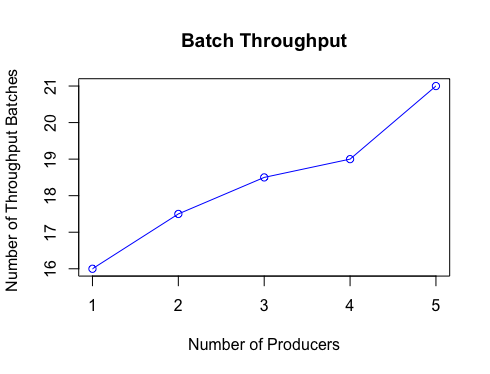
\includegraphics[width=0.5\textwidth]{./images/throughput.png}
        \caption{Query 2 throughput for different number of Producers. (Batch Size 1k)}
        \label{fig:evaluation}
    \end{center}
\end{figure}


%TODO!: Experiment with different architectures if we have any. 


\section{Conclusion}\label{sec:conclustion}








\bibliographystyle{ACM-Reference-Format}
\bibliography{references}


\end{document}
\endinput
